\chapter{MARCO METODOLÓGICO}
\label{cap:metodologia}

Este capítulo describe GBMARL, el marco de aprendizaje por refuerzo multiagente adversarial propuesto para descubrir políticas de dosificación adaptativa en glioblastoma. La construcción sigue un principio de validación incremental, de adentro hacia afuera: primero se especifica y prueba el simulador de la dinámica tumoral (Sección~\ref{sec:simulador}); luego se calibra con datos reales de sensibilidad farmacológica (Sección~\ref{sec:calibracion}); a continuación se formula el problema de decisión como un juego adversarial de dos agentes (Sección~\ref{sec:juego}) con una función de recompensa alineada al desenlace clínico (Sección~\ref{sec:recompensa}); se entrena mediante el algoritmo MAPPO con entrenamiento centralizado y ejecución descentralizada (Sección~\ref{sec:algoritmo}); y, finalmente, se evalúa bajo un protocolo experimental con una métrica de progresión auditada (Sección~\ref{sec:protocolo}).

Este orden no es accidental: la ecuación diferencial es comprobable de forma aislada, y un agente único entrenado con PPO contra un tumor de comportamiento fijo permite verificar el entorno antes de introducir la complejidad del aprendizaje multiagente.

\section{Visión general del marco}
\label{sec:vision-general}

GBMARL modela el tratamiento del glioblastoma como un juego de suma no nula entre dos agentes que actúan sobre un mismo sistema dinámico:

\begin{itemize}
  \item El \textbf{agente de terapia} elige, en cada paso de decisión, la tasa de administración del fármaco $u(t)$; su objetivo es maximizar el tiempo durante el cual el tumor permanece clínicamente manejable.
  \item El \textbf{agente tumoral} controla la tasa de transición fenotípica $\phi$ de células sensibles a resistentes; su objetivo es forzar la dominancia de la población resistente.
\end{itemize}

Ambos agentes aprenden simultáneamente mediante \emph{self-play} sobre un simulador de ecuaciones diferenciales ordinarias (EDO). Es crucial subrayar que los datos experimentales \emph{solo calibran el simulador}: no se entrena ninguna red supervisada sobre datos de pacientes. Las políticas emergen de la interacción con el simulador calibrado, lo que sitúa el aprendizaje en un régimen de control óptimo bajo incertidumbre evolutiva, en lugar de un régimen de predicción supervisada.

\section{Simulador de la dinámica tumoral}
\label{sec:simulador}

El tumor se representa mediante dos poblaciones celulares en competencia: las sensibles $S$ y las resistentes $R$, junto con la concentración intratumoral del fármaco $c$. La dinámica sigue un modelo de competición logística tipo Lotka-Volterra acoplado a la farmacodinámica del fármaco~\cite{Strobl2020,Yin2019}:

\begin{align}
  \frac{dS}{dt} &= \alpha_S\, S\left(1 - \frac{S+R}{K}\right) - \delta_S(c)\,S - \phi\,S, \label{eq:ode-S}\\[4pt]
  \frac{dR}{dt} &= \alpha_R\, R\left(1 - \frac{S+R}{K}\right) - \delta_R(c)\,R + \phi\,S, \label{eq:ode-R}\\[4pt]
  \frac{dc}{dt} &= -\lambda_c\, c + u(t). \label{eq:ode-c}
\end{align}

Aquí $\alpha_S$ y $\alpha_R$ son las tasas de crecimiento intrínsecas, $K$ la capacidad de carga, y $\lambda_c$ la tasa de eliminación del fármaco. El término $\phi\,S$ representa la conversión fenotípica de sensibles a resistentes: aparece restado en~\eqref{eq:ode-S} y sumado en~\eqref{eq:ode-R}, lo que conserva la masa celular transferida. Modelar la resistencia como una transición fenotípica controlable ---y no como una mutación irreversible--- está respaldado por la evidencia de plasticidad fenotípica reversible en la resistencia no genética~\cite{Boumahdi2019}.

El efecto citotóxico del fármaco sobre cada población se modela con una función de Hill, que captura la respuesta sigmoide dosis-efecto característica de los ensayos de sensibilidad:

\begin{equation}
  \delta_X(c) = \delta_X^{\max}\, \frac{c^{\,h}}{\mathrm{IC50}_X^{\,h} + c^{\,h}}, \qquad X \in \{S, R\}, \label{eq:hill}
\end{equation}

donde $\delta_X^{\max}$ es la muerte celular máxima alcanzable, $\mathrm{IC50}_X$ la concentración que produce la mitad del efecto máximo, y $h$ el coeficiente de Hill. La diferencia clave entre poblaciones reside en que $\mathrm{IC50}_R \gg \mathrm{IC50}_S$: las células resistentes requieren concentraciones mucho mayores para ser afectadas.

El sistema~\eqref{eq:ode-S}--\eqref{eq:ode-c} se integra numéricamente mediante el método de Runge-Kutta de cuarto orden (RK4) con paso fijo $dt$. La implementación de la dinámica es matemática pura y se valida de forma aislada mediante pruebas unitarias: en ausencia de fármaco el tumor crece hasta la capacidad de carga; bajo dosis alta constante la población sensible decrece y la resistente se expande; y las poblaciones nunca toman valores negativos.

\section{Calibración del simulador con datos reales}
\label{sec:calibracion}

La calibración separa estrictamente lo que proviene de los datos de lo que proviene de la literatura. El principio rector es que \emph{los datos determinan la potencia del fármaco} (la posición de las curvas dosis-respuesta y la brecha de sensibilidad entre poblaciones), mientras que \emph{la literatura ancla el techo de muerte y las tasas de crecimiento}.

\subsection{Fuente y procesamiento de datos}

Las concentraciones inhibitorias se derivan de los ensayos de sensibilidad a temozolomida en líneas celulares de glioblastoma del repositorio GDSC2~\cite{GDSC}, cruzados con la anotación genómica de DepMap~\cite{DepMap}. El cruce entre ambos repositorios es un punto crítico: las claves de identificación deben normalizarse en ambos lados (mayúsculas y eliminación de caracteres no alfanuméricos) antes del mapeo, pues un cruce ingenuo por nombre pierde líneas en silencio. Tras la corrección, se recuperan 34 líneas de glioblastoma con ensayos de sensibilidad y 24 con genómica completa, frente a las 6 que recuperaba la versión defectuosa del cruce. Este saneamiento se documenta reportando explícitamente cuántas líneas se recuperan y por qué se descarta cada una.

De estos datos se estima la $\mathrm{IC50}$ de la población sensible y, a partir de la dispersión de respuestas, la $\mathrm{IC50}$ efectiva de la población resistente. El resultado es una brecha de sensibilidad de aproximadamente un orden de magnitud ($\mathrm{IC50}_R / \mathrm{IC50}_S \approx 9$), coherente con el carácter clínicamente refractario del glioblastoma a la temozolomida.

\subsection{Procedencia de los parámetros}

El techo de muerte $\delta_X^{\max}$ no se estima de datos \emph{in vitro} ---que no informan directamente la dinámica de competencia--- sino que se ancla a la literatura mediante una razón muerte-crecimiento, $\delta_S^{\max} = \kappa\, \alpha_S$ con $\kappa = 2{,}0$, garantizando que el fármaco disponga de palanca terapéutica suficiente. La Tabla~\ref{tab:procedencia} documenta la procedencia de cada parámetro, distinguiendo entre los derivados de \textbf{datos}, los anclados a \textbf{literatura}, y los fijados por \textbf{normalización} del modelo.

\begin{table}[H]
\centering
\caption{Procedencia de los parámetros del simulador. DATO: estimado de GDSC2/DepMap; LIT: anclado a literatura; NORM: fijado por normalización del modelo.}
\label{tab:procedencia}
\renewcommand{\arraystretch}{1.2}
\begin{tabular}{l|l|c|l}
\textbf{Parámetro} & \textbf{Símbolo} & \textbf{Valor} & \textbf{Procedencia} \\
\hline
Crecimiento sensibles      & $\alpha_S$        & 0.15  & LIT \\
Crecimiento resistentes    & $\alpha_R$        & 0.10  & LIT (costo de resistencia) \\
Capacidad de carga         & $K$               & 1.0   & NORM \\
Eliminación del fármaco    & $\lambda_c$       & 0.40  & LIT \\
Transición basal           & $\phi_{\text{base}}$ & 0.005 & LIT \\
IC50 sensibles             & $\mathrm{IC50}_S$ & 0.36  & DATO (GDSC2) \\
IC50 resistentes           & $\mathrm{IC50}_R$ & 3.27  & DATO (GDSC2) \\
Coeficiente de Hill        & $h$               & 2.0   & LIT \\
Muerte máx.\ sensibles     & $\delta_S^{\max}$ & 0.30  & LIT (anclada, $\kappa\,\alpha_S$) \\
Muerte máx.\ resistentes   & $\delta_R^{\max}$ & 0.15  & LIT (anclada) \\
\end{tabular}
\end{table}

Toda fórmula que transforma un dato en un parámetro de la EDO queda documentada de forma explícita, sin constantes mágicas sin derivación. Un hallazgo honesto de la calibración es que la temozolomida resulta un fármaco débil \emph{in vitro}, lo cual refleja fielmente la realidad clínica del glioblastoma como enfermedad incurable.

\section{Formulación como juego adversarial multiagente}
\label{sec:juego}

El problema de decisión se formula como un entorno multiagente paralelo siguiendo la interfaz \texttt{ParallelEnv} de PettingZoo~\cite{Terry2021}, con dos agentes que actúan de manera simultánea sobre el sistema~\eqref{eq:ode-S}--\eqref{eq:ode-c}. El estado dinámico real del sistema es tridimensional, $s = (S, R, c)$; los descriptores genómicos de la línea celular condicionan los parámetros iniciales a través de la calibración, pero no evolucionan durante el episodio.

\subsection{Observabilidad parcial}

Un elemento central del diseño es la observabilidad parcial clínicamente justificada. El agente de terapia no observa la composición interna del tumor, sino únicamente la carga total y la concentración del fármaco, replicando la limitación real del oncólogo, que no puede medir directamente la fracción resistente:

\begin{equation}
  o^{\text{ter}} = (S+R,\; c), \qquad o^{\text{tum}} = (S,\; R), \qquad s^{\text{global}} = (S, R, c). \label{eq:obs}
\end{equation}

Esta asimetría informativa es precisamente lo que motiva un crítico centralizado: durante el entrenamiento, el crítico puede acceder al estado conjunto $s^{\text{global}}$ ---incluida la fracción resistente que el actor de terapia no observa--- para realizar una mejor asignación de crédito.

\subsection{Espacios de acción}

La acción del agente de terapia es la tasa de dosificación $u \in [0, u_{\max}]$. La acción del agente tumoral es la tasa de transición fenotípica $\phi \in [0, \phi_{\max}]$. Acotar la acción del adversario es esencial: un adversario sin restricción puede forzar trivialmente la resistencia y degenerar en un \emph{hombre de paja} sin valor de modelado. La cota $\phi_{\max}$ y el costo de crecimiento implícito (la conversión drena la población sensible) imponen un compromiso evolutivo realista al tumor.

\section{Diseño de la función de recompensa}
\label{sec:recompensa}

El diseño de la recompensa fue iterativo y constituye, en sí mismo, un resultado metodológico. Documentamos su evolución de forma honesta porque ilustra una trampa conceptual recurrente.

\subsection{Evolución de la recompensa}

Una primera recompensa que penalizaba la carga tumoral instantánea ($r^{\text{ter}} = -(S+R)$) condujo al agente a redescubrir la estrategia de dosis máxima: minimizar la carga a corto plazo selecciona agresivamente la resistencia y pierde a largo plazo. Penalizar la fracción resistente con un peso fijo tampoco resolvió el problema: un peso alto hacía al agente abandonar el control de la carga, y un peso bajo lo hacía ignorar la resistencia. La lección es que \emph{minimizar el tamaño del tumor es el objetivo equivocado}; el objetivo correcto es maximizar el tiempo durante el cual el tumor permanece simultáneamente controlado y tratable.

\subsection{Recompensa final}

La formulación final premia directamente cada día de manejo clínico exitoso. Definimos dos condiciones sobre el estado:

\begin{align}
  \text{controlado} &: \quad S + R < \theta_{\text{prog}}, \label{eq:controlado}\\
  \text{tratable}   &: \quad \frac{R}{S+R} < \rho_{\text{may}}, \label{eq:tratable}
\end{align}

donde $\theta_{\text{prog}} = 0{,}8\,K$ es el umbral de progresión en carga y $\rho_{\text{may}} = 0{,}5$ el umbral de mayoría resistente. La recompensa del agente de terapia otorga una bonificación por cada día en que ambas condiciones se cumplen, menos un costo de toxicidad proporcional a la dosis:

\begin{equation}
  r^{\text{ter}} = b_{\text{ctrl}}\cdot \mathbb{1}[\text{controlado} \wedge \text{tratable}] - w_{\text{tox}}\, u, \label{eq:reward-ter}
\end{equation}

y el agente tumoral recibe una recompensa creciente con la fracción resistente más una bonificación al forzar la falla:

\begin{equation}
  r^{\text{tum}} = \frac{R}{S+R} + b_{\text{prog}}\cdot \mathbb{1}[\neg(\text{controlado} \wedge \text{tratable})]. \label{eq:reward-tum}
\end{equation}

El episodio termina cuando falla cualquiera de las dos condiciones, o por erradicación (con una bonificación $b_{\text{win}}$ para la terapia), o por truncamiento al alcanzar el horizonte. La Tabla~\ref{tab:hiperparametros-env} resume los valores adoptados.

\begin{table}[H]
\centering
\caption{Hiperparámetros del entorno y de la recompensa.}
\label{tab:hiperparametros-env}
\renewcommand{\arraystretch}{1.2}
\begin{tabular}{l|c||l|c}
\textbf{Parámetro} & \textbf{Valor} & \textbf{Parámetro} & \textbf{Valor} \\
\hline
Bonif.\ de control $b_{\text{ctrl}}$       & 1.0  & Umbral progresión $\theta_{\text{prog}}$ & $0.8\,K$ \\
Peso de toxicidad $w_{\text{tox}}$         & 0.05 & Umbral mayoría $\rho_{\text{may}}$        & 0.50 \\
Bonif.\ progresión $b_{\text{prog}}$       & 10.0 & Cota de transición $\phi_{\max}$          & 0.05 \\
Bonif.\ erradicación $b_{\text{win}}$      & 50.0 & Horizonte (días)                          & 180 \\
Estado inicial $S_0,\,R_0$                 & 0.40,\,0.01 & Paso de integración $dt$           & 0.1 \\
\end{tabular}
\end{table}

\section{Algoritmo de aprendizaje: MAPPO-CTDE}
\label{sec:algoritmo}

Las políticas se aprenden con una implementación propia en PyTorch de \emph{Multi-Agent Proximal Policy Optimization} (MAPPO)~\cite{Yu2022}, bajo el paradigma de entrenamiento centralizado y ejecución descentralizada (CTDE)~\cite{Amato2024}. Cada agente $i$ posee un actor $\pi_{\theta_i}(a^i \mid o^i)$ que actúa sobre su observación local, y comparte el marco de optimización de PPO~\cite{Schulman2017}.

\subsection{Crítico centralizado y estimación de ventajas}

El componente CTDE reside en el crítico. En la variante MAPPO, el crítico $V_{\psi_i}(s^{\text{global}})$ de cada agente accede al estado conjunto~\eqref{eq:obs} durante el entrenamiento, mientras que los actores ejecutan solo con su observación local. Las ventajas se estiman mediante \emph{Generalized Advantage Estimation} (GAE)~\cite{Schulman2016}:

\begin{equation}
  \hat{A}_t = \sum_{l=0}^{T-t-1} (\gamma\lambda)^l\, \delta_{t+l}, \qquad \delta_t = r_t + \gamma V_\psi(s_{t+1}) - V_\psi(s_t), \label{eq:gae}
\end{equation}

y cada actor se actualiza con el objetivo recortado de PPO:

\begin{equation}
  \mathcal{L}^{\text{PPO}}(\theta) = \mathbb{E}_t\!\left[\min\left(\varrho_t(\theta)\,\hat{A}_t,\; \mathrm{clip}(\varrho_t(\theta), 1-\epsilon, 1+\epsilon)\,\hat{A}_t\right)\right] + c_{\text{ent}}\, \mathcal{H}[\pi_\theta], \label{eq:ppo}
\end{equation}

donde $\varrho_t(\theta)$ es el cociente de probabilidades entre la política nueva y la antigua, y $\mathcal{H}$ el término de entropía que favorece la exploración. La naturaleza adversarial se introduce mediante \emph{self-play}: ambos agentes se entrenan simultáneamente, cada uno optimizando su propia recompensa contra la política actual del oponente, un esquema cuya estabilidad y robustez están respaldadas por el aprendizaje por refuerzo adversarial robusto~\cite{Pinto2017}.

\subsection{Variante de ablación: IPPO}

Para aislar empíricamente la contribución del crítico centralizado, se implementa la variante de aprendizaje independiente (IPPO)~\cite{deWitt2020}, idéntica en todo salvo en que el crítico $V_{\psi_i}(o^i)$ observa únicamente la observación local del agente, en lugar del estado conjunto. La comparación entre ambas variantes, manteniendo fijos el actor, la observación de ejecución y todos los hiperparámetros, aísla el efecto puro de CTDE.

\begin{algorithm}[H]
\SetAlgoLined
\KwIn{simulador calibrado, semilla, número de pasos $N$, modo (MAPPO/IPPO)}
\KwOut{políticas $\pi_{\theta_{\text{ter}}}$, $\pi_{\theta_{\text{tum}}}$}
Inicializar actores y críticos; fijar semillas y modo determinista\;
\While{pasos $< N$}{
  Recolectar trayectorias de \emph{self-play}: ambos agentes actúan sobre el simulador\;
  \For{cada agente $i \in \{\text{terapia}, \text{tumor}\}$}{
    Entrada del crítico $\gets s^{\text{global}}$ si MAPPO, o $o^i$ si IPPO\;
    Calcular ventajas $\hat{A}_t$ con GAE según~\eqref{eq:gae}\;
    Actualizar actor con el objetivo recortado~\eqref{eq:ppo} y crítico por regresión de valor\;
  }
}
\caption{Entrenamiento adversarial por self-play (MAPPO / IPPO).}
\label{alg:selfplay}
\end{algorithm}

\subsection{Reproducibilidad}

Dado que el entrenamiento adversarial por \emph{self-play} es intrínsecamente inestable y puede asentarse en distintos equilibrios según la inicialización, se impone un régimen determinista: ejecución en un solo hilo, activación de algoritmos deterministas y sembrado completo de los generadores aleatorios. Esto garantiza que una misma semilla produzca el mismo resultado dentro de un experimento, a costa de la velocidad de cómputo.

\section{Protocolo experimental y métricas de evaluación}
\label{sec:protocolo}

\subsection{Métrica de progresión auditada}

El desenlace se mide con el \textbf{tiempo a falla combinado} (TTP-combinado): el número de días hasta que el tumor deja de estar controlado~\eqref{eq:controlado} \emph{o} deja de ser tratable~\eqref{eq:tratable}, lo que ocurra primero, reportando además el \emph{motivo} de falla (progresión en carga, mayoría resistente o supervivencia al horizonte). Esta métrica es clínicamente honesta por construcción y evita un artefacto sutil: una métrica basada únicamente en la resistencia asignaría falsamente el valor del horizonte a un episodio que en realidad falló por progresión de carga, inflando los resultados. Toda evaluación reporta el modo de falla para permitir su auditoría.

\subsection{Líneas base y validación}

La política aprendida se compara contra tres referencias deterministas evaluadas sobre el mismo simulador y bajo la misma métrica: la ausencia de tratamiento ($u \equiv 0$), la dosis máxima tolerada ($u \equiv u_{\max}$), y la terapia adaptativa heurística de Gatenby (dosificación de encendido/apagado según umbrales de carga)~\cite{Gallaher2017,Stankova2019}. La validación se realiza sobre múltiples semillas independientes; dado que el \emph{self-play} produce resultados bimodales, los resultados se reportan por tasa de éxito y mediana, en lugar de promedios que serían engañosos para una distribución bimodal, y la significancia frente a las líneas base se contrasta con pruebas apropiadas para varianza no homogénea.

\subsection{Estudios de ablación y sensibilidad}

Dos estudios complementan la validación principal. El \textbf{estudio de ablación} compara MAPPO (crítico centralizado) frente a IPPO (crítico local) sobre las mismas semillas, aislando la contribución de CTDE. El \textbf{análisis de sensibilidad} varía, una a la vez, las constantes elegidas a mano ---la fuerza del adversario $\phi_{\max}$, los umbrales de evaluación $\theta_{\text{prog}}$ y $\rho_{\text{may}}$, el peso de toxicidad $w_{\text{tox}}$, la potencia del fármaco $\delta_S^{\max}$ y la brecha de resistencia $\mathrm{IC50}_R$--- alrededor de su valor por defecto, para verificar que el ordenamiento entre estrategias es robusto y no depende de la elección particular de hiperparámetros. Los resultados de ambos estudios se presentan en el Capítulo~\ref{cap:resultados}.

\section{Pipeline experimental reproducible}
\label{sec:pipeline}

Las secciones anteriores describen los componentes de GBMARL de forma aislada. En la práctica, esos componentes se ejecutan como un \textbf{pipeline único, reproducible y construido de adentro hacia afuera} (\emph{inside-out}), en el que cada fase \emph{de-riskea} a la siguiente: ninguna etapa se da por válida hasta que la anterior ha sido verificada. La Figura~\ref{fig:pipeline} resume las siete fases y su encadenamiento; la decisión de ordenarlas así responde a una estrategia de control de riesgo, no a una conveniencia de implementación.

\begin{figure}[H]
\centering
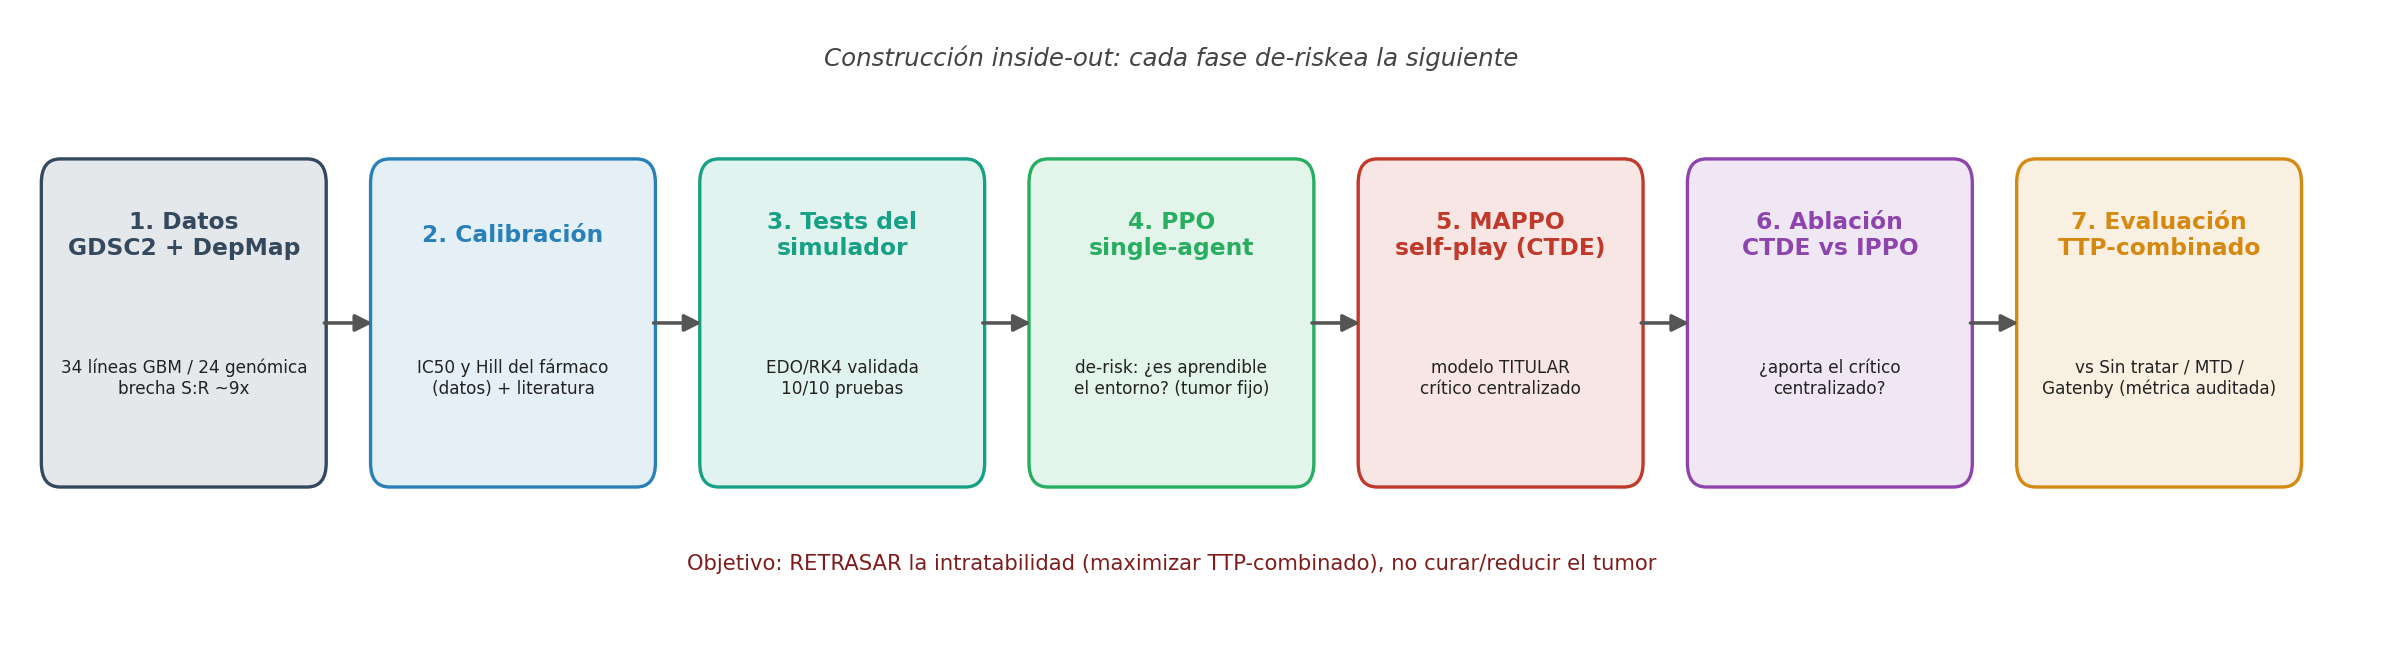
\includegraphics[width=\textwidth]{images/pipeline_diagram.png}
\caption{Pipeline experimental reproducible de GBMARL. Cada fase de-riskea la siguiente: los datos calibran el simulador, el simulador se valida con pruebas unitarias, un agente único (PPO) confirma que el entorno es aprendible antes de introducir el segundo agente, el modelo titular (MAPPO) se contrasta con su ablación (IPPO) y, finalmente, todo se evalúa con la métrica auditada frente a las líneas base. El objetivo transversal es \emph{retrasar} la intratabilidad, no reducir el tumor.}
\label{fig:pipeline}
\end{figure}

La Tabla~\ref{tab:pipeline} explicita, para cada fase, su propósito, su vínculo con el objetivo clínico (maximizar el tiempo de manejo) y qué aporta o qué riesgo elimina dentro del marco. La lógica de fondo es que un resultado multiagente solo es creíble si el sustrato sobre el que se aprende ---la dinámica, su calibración y la propia aprendibilidad del entorno--- ya fue probado por separado.

\begin{table}[H]
\centering
\caption{Fases del pipeline experimental: propósito, vínculo con el objetivo y contribución. El objetivo del marco es maximizar el TTP-combinado (retrasar la intratabilidad).}
\label{tab:pipeline}
\renewcommand{\arraystretch}{1.3}
\begin{tabular}{p{2.4cm}|p{4.0cm}|p{5.7cm}}
\textbf{Fase} & \textbf{Propósito} & \textbf{Vínculo con el objetivo y contribución} \\
\hline
1. Datos (GDSC2 + DepMap) & Recuperar líneas de glioblastoma con sensibilidad a temozolomida. & Anclan la dinámica a la biología real (brecha S:R $\approx 9\times$); sin ellos la resistencia sería un supuesto arbitrario. \\
2. Calibración & Derivar IC50 y forma de Hill de los datos; anclar el resto a literatura. & Fija la \emph{potencia} del fármaco con la que se mide cuánto se puede retrasar la progresión; separa dato de supuesto. \\
3. Tests del simulador & Probar la EDO/RK4 de forma aislada (10/10 pruebas). & Garantiza que la dinámica conserva masa y es biológicamente válida antes de aprender sobre ella. \\
4. PPO single-agent & De-riskear el entorno: ¿es aprendible contra un tumor fijo? & Verifica que la señal de recompensa induce control \emph{antes} de añadir el adversario; aísla fallos del entorno de fallos del MARL. \\
5. MAPPO self-play (CTDE) & Entrenar el modelo titular: terapia y tumor co-evolucionan. & Produce la política adaptativa que maximiza el tiempo de manejo; es la contribución central. \\
6. Ablación CTDE vs.\ IPPO & Aislar el efecto del crítico centralizado. & Atribuye causalmente la ventaja al componente CTDE, no al azar ni a otros factores. \\
7. Evaluación TTP-combinado & Comparar frente a Sin tratar, MTD y Gatenby con la métrica auditada. & Cuantifica el objetivo (días de manejo) de forma honesta y comparable; cierra el ciclo de validación. \\
\end{tabular}
\end{table}

\subsection{Por qué cada comparación}
\label{sec:porque-comparaciones}

El pipeline contiene tres comparaciones deliberadas, cada una respondiendo a una pregunta distinta. La comparación frente a las \textbf{líneas base} (Sin tratamiento, MTD y Gatenby) responde a si el aprendizaje aporta algo sobre lo ya conocido: Sin tratamiento fija el piso (la progresión natural), MTD representa el estándar clínico intuitivo de ``pegar fuerte'' y Gatenby es el competidor fuerte ---la mejor heurística adaptativa publicada---, de modo que superar a Gatenby es la prueba exigente de valor. La comparación \textbf{MAPPO frente a IPPO} (ablación) responde a si el crítico centralizado es la causa de la ventaja, manteniendo todo lo demás idéntico; sin esta comparación, atribuir el resultado a CTDE sería una conjetura. La comparación de \textbf{PPO frente al azar} (de-risk) responde a si el entorno es siquiera aprendible, y debe pasar antes de invertir esfuerzo en el aprendizaje multiagente. Reportar las tres ---y no solo la favorable--- es lo que convierte el resultado en una afirmación auditable.

\subsection{Ejecución reanudable con checkpointing intra-corrida}
\label{sec:checkpointing}

El entrenamiento adversarial a la escala de la tesis (120\,000 pasos por corrida, decenas de semillas entre el modelo titular y la ablación) excede el tiempo disponible en una sola ejecución del entorno de cómputo. Para preservar la reproducibilidad sin sacrificar la escala, el pipeline se ejecuta mediante un \textbf{arnés reanudable con checkpointing intra-corrida}: cada ventana de cómputo entrena durante un presupuesto fijo de tiempo y luego serializa un punto de control completo ---pesos de actores y críticos, estado de los optimizadores, estado de los generadores aleatorios, paso acumulado y estado del entorno---, de modo que la siguiente ventana reanuda exactamente donde la anterior se detuvo, hasta alcanzar los pasos objetivo. El rollout de entrenamiento emplea además una ruta de integración escalar de la EDO, verificada numéricamente como idéntica a la implementación vectorizada de referencia (diferencia máxima nula sobre trayectorias completas), que reduce el tiempo de cómputo sin alterar la física ni la recompensa. Este mecanismo no modifica ninguna decisión de modelado: es la maquinaria de ejecución que hace factible la corrida completa de validación reportada en la Sección~\ref{sec:res-confirmacion}.